Hasta donde sabemos, el mundo consiste de part\'iculas elementales, que
son indivisibles, y occurren en pocos tipos (decimos 25, pero depende
un poco de como se cuenta). Ejemplos famosos son el electr\'on y el
fot\'on (la part\'icula de la luz).

Su descripci\'on relativista funciona con ``campos'', objetos
abstractos, presentes en todo el universo, en cualquier momento.
En un punto, un campo puede tomar diferentes estados, que dependen
del tiempo. Si los campos en una regi\'on est\'an en su estado base,
percibimos el vac\'io. Las excitaciones son cu\'antizadas y se
manifiestan como part\'iculas elementales -- esto es la idea de la
{\it teor\'ia cu\'antica de campos.}

Existe un campo para cada tipo de part\'icula elemental,
y sus excitaciones pueden moverse (como ondas), interactuar,
generar y destruir part\'iculas (esto es un requisito para
la compatibilidad con la Relatividad Especial, que falta en
la mec\'anica cu\'antica).\footnote{Ref. \cite{WBparti} presenta
  otra explicaci\'on divulgativa pero m\'as extensa.}

Un concepto central son las simetr\'ias: una simetr\'ia significa
la invarianza de las propiedades f\'isicas bajo un grupo de
transformaciones de uno o varios campos. Distinguimos simetr\'ias
{\em globales} y {\em locales:}

\begin{itemize}

\item En una simetr\'ia {\em global,} un campo se transforma de la
  misma manera en todas partes. Se puede imaginar un grupo de personas
  que hacen gimnasia colectiva, todas hacen el mismo movimiento,
  puede ser sincronizado con m\'usica.
  (La imagen es un poco simplista porque los campos se transforman
  de la misma manera incluso en todo el espacio-tiempo.)
  
\item El caso de una simetr\'ia {\em local} se puede imaginar como
  gimnasia ca\'otica: cada persona se mueve como quiere, de manera
  independiente. Esto significa que los campos pueden ser transformados
  independientemente en cada punto del espacio-tiempo.

  Es claro que este tipo de simetr\'ia permite muchas m\'as
  transformaciones.
  Lograr una simetr\'ia local es m\'as dif\'icil, pero conduce
  a restricciones m\'as fuertes, y por lo tanto a una poderosa
  capacidad de hacer predicciones.
  
  T\'ecnicamente, se introduce un campo adicional, conocido como
  ``campo de norma'', que transforma tal que compensa el cambio
  relativo entre puntos cercanos en una transformaci\'on simult\'anea.
  Este concepto exitoso describe la transmisi\'on de interacciones,
  pero solamente funciona si la simetr\'ia local es exacta.
  
\end{itemize}

Una categor\'ia importante de part\'iculas es conocida como
``fermiones'': los fermiones elementales (conocidos) tienen
``esp\'in $1/2 $'' en unidades naturales.\footnote{Para
usar unidades naturales, se coloca la constante
cu\'antica de Planck y la velocidad de la luz en el vac\'io a 1,
$\hbar = c =1$.}
El esp\'in es un grado de libertad interno que se manifesta como
momento angular. Ejemplos para fermiones son el electr\'on, sus dos
``primos'' m\'as pesados (el mu\'on y el tau\'on), los neutrinos (mucho
m\'as ligeros y sin carga el\'ectrica)\footnote{El conjunto del
electr\'on, mu\'on, tau\'on y los tres neutrinos es conocido como
los {\em leptones}.}
y los cuarks (constituyentes
de part\'iculas compuestas, como el prot\'on y el neutr\'on).

Un fermi\'on puede existir en dos variantes, con ``quiralidad''
izquierda o derecha; se pude imaginar como manos,\footnote{Efectivamente,
el t\'ermino viene de ``kheir'', que significa ``mano'' en griego.} 
o guantes, izquierdo o derecho, pero en un sentido abstracto.

Suponemos por ejemplo un electr\'{o}n sin masa: en este caso,
el electr\'on izquierdo ($e_L$) y derecho ($e_R$) son independientes,
y su esp\'in apunta contra (para $e_L$) o en (para $e_R$) la
direcci\'on de su movimiento (una part\'icula sin masa no
puede estar en reposo). Esto es ilustrado simbolicamente en
la Figura \ref{electron}.

\begin{figure}
\centering
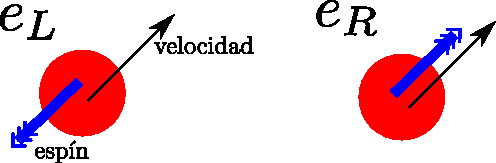
\includegraphics[scale=1]{images/quiral.pdf}
\caption{Representaci\' on simb\'olica de un electr\'on sin masa con
quiralidad izquierda $e_L$ (izquierda) y quiralidad derecha $e_R$
(derecha). La direcci\'on del movimiento es
indicada por la flecha delgada y la direcci\'on del esp\'in
por la flecha gruesa. Para quiralidad izquierda velocidad y
esp\'in apuntan en direcciones contrarias, pero para la quiralidad
derecha apuntan en la misma direcci\'on.}
\label{electron}
\end{figure}
Incluir un t\'ermino de masa requiere de un producto de los campos
del electr\'on izquierdo y derecho (se puede imaginar que las dos
manos se agarran). Entonces ya no son independientes, y bajo una
simetr\'ia tienen que transformarse de la misma manera.

Sin embargo, esto no es el caso en la teor\'ia electrod\'ebil de Glashow
\cite{Glashow}: esta teor\'ia permite, por ejemplo, transformaciones
locales (``de norma'') que solamente afectan al $e_L$, pero no al $e_R$.
Aqu\'i era el problema: dicha teor\'ia pareci\'o ser incompatible con
el t\'ermino de masa del electr\'on (y de otros fermiones), pero sabemos
que el electron s\'i tiene una masa de $M_e \simeq 0.511\ {\rm MeV}$
(todav\'ia en unidades naturales).

De hecho, la situaci\'on era a\'un peor. Las part\'iculas de norma
que transmiten la fuerza d\'ebil se llaman $W^{\pm}$, $Z^0$
(con carga el\'ectrica $\pm1, \, 0$), por ejemplo los $W$ son
responsables del decaimiento radioactivo. Esta fuerza tiene un
alcance muy corto (como $10^{-17}$~m) que solamente se puede
explicar si $W^{\pm}$, $Z^0$ tienen masas grandes (est\'an entre
las part\'iculas elementales m\'as pesadas que conocemos, con
masas de $M_W = 80.4 \, {\rm GeV}$ y $M_Z = 91.2\,{\rm GeV}$). 
Pero igual que la masa del electr\'on, parece que la simetr\'ia
de norma -- que tiene que ser exacta -- requiere $m_W = m_Z = 0$.

El acertijo de d\'onde pueden venir estas masas de part\'iculas
de norma era una ``pregunta matadora'' con la cual Wolfgang Pauli
destruy\'o un seminario de Chen-Ning Yang en Princeton en 1953
sobre teor\'ias de
norma con un grupo de simetr\'ia no abeliano (ahora conocidas como
teor\'ias de Yang-Mills). Sin conocer el mecanismo de Higgs, Yang no
logr\'o contestar, pero Pauli insisti\'o tanto hasta
que Yang se sent\'o frustrado. Finalmente Robert Oppenheimer tuvo
que animarlo para continuar su charla \cite{Shifman}.

Entonces, ?`c\'omo funciona la salvaci\'on de esta teor\'ia,
el mecanismo de Higgs? Primero, se agrega otro campo m\'as,
el {\em campo de Higgs}, usamos la notaci\'on $\phi (x)$.
La variable $x$ es un punto del espacio-tiempo, y $\phi$ es
un campo escalar, sus fluctuaciones representan part\'iculas 
con esp\'in 0. Para establecer un t\'ermino de masa del electr\'on,
ahora se forma un producto de {\em tres} campos, $e_L$, $\phi$ y
$e_R$.\footnote{Realmente necesitamos parcialmente anti-campos,
que representan anti-part\'iculas, pero ignoramos
este aspecto en el contexto de este art\'iculo de divulgaci\'on.}
El campo de Higgs tambi\'en transforma bajo la simetr\'ia local,
de tal manera que el t\'ermino en su totalidad s\'i es invariante
de norma.

Entonces de esta manera se puede agregar un t\'ermino permitido
(invariante de norma), pero ?`esto proporciona una masa al electr\'on?
Posiblemente s\'i, puede funcionar con el escenario siguiente.

A bajas energ\'ias, el campo de Higgs ``se congela'' en su estado
base, se manifiesta casi como una constante. Esta constante no
tiene que ser cero: realmente $\phi$ tiene 4 componentes reales, pero
nos podemos imaginar que sean 2 solamente,
$\phi_1 , \, \phi_2 \in \R$, que parametrizan un plano.
Este campo viene con un potencial $V(\phi_1, \phi_2)$ de la forma
de un sombrero, con el valor cero al centro, pero hay un anillo
de m\'inimos que corresponden a un valor
$|\phi|^2 = \phi_1^2 + \phi_2^2 > 0$, como est\'a ilustrado en la
Figura \ref{sombrero}.
Este ``valor esperado en el vac\'io'' toma el papel de la masa
del electr\'on que el modelo necesita (hasta un coeficiente),
$M_e \propto |\phi|$, y de manera an\'aloga tambi\'en se obtienen
las masas $M_W$ y $M_Z$, todos conforme a la simetr\'ia de norma
(regresaremos a este tema).

Parece todo bien, pero hay otro problema todav\'ia, y a esto
Coleman se refiri\'o en su comentario sobre el seminario de
Higgs en Harvard, que hemos mencionado en Secci\'on 1.

El potencial sombrero tiene una simetr\'ia bajo rotaciones por
el centro. Suponemos que el campo $\phi$ elige uno de
los m\'inimos: el proceso de esta elecci\'on se denota como
``rompimiento espont\'aneo de la simetr\'ia'': desde
la perspectiva de un m\'inimo espec\'ifico, ya no se ve la
simetr\'ia de rotaci\'on. En Ref.\ \cite{HiggsBol} hemos
descrito este proceso con la analog\'ia del {\em Asno de Buridan,}
que est\'a sediento y rodeado por un abrevadero de agua, pero
tiene que decidirse en que direcci\'on camina para beber agua.

Peque\~nas fluctuaciones del campo m\'as all\'a de su estado
m\'inimo corresponden a part\'iculas. Si una fluctuacion es
{\em radial,} cuesta energ\'ia porque el potencial sube -- esto
es una part\'icula masiva (la curvatura del potencial en la
direcci\'on radial corresponde a la masa en cuadrado.)
Por otro lado, una fluctuaci\'on {\em tangencial} no necesita
energ\'ia, pues el campo se queda con energ\'ia m\'inima.
Esto es un ejemplo de una part\'icula sin masa, conocido
como un {\em bos\'on de Nambu-Goldstone} \cite{Nambu,Goldstone}.
Seg\'un el Teorema de Goldstone \cite{GSW}, estos bosones aparecen
cuando una simetr\'a continua (como la rotaci\'on en este
ejemplo) se rompe espont\'aneamente.

Si el mecanismo funciona como descrito antes, se queda la
pregunta: ?`d\'onde est\'a este bos\'on de Nambu-Goldstone?
Por ser sin masa, tendr\'a que tomar un papel importante
y dominar la f\'isica a bajas energ\'ias (donde part\'iculas
muy pesadas no se manifiestan). Pero ninguna part\'icula de
este estilo fue observada. Entonces para justificar el mecanismo,
se tiene que ``evadir el Teorema de Goldstone'', como dijo
Coleman, y sus colegas en Harvard dudaron si esto es posible.
No eran los \'unicos, por ejemplo Klaus Hepp, prominente
f\'isico matem\'atico, advirti\'o a Higgs que esto no podr\'ia
funcionar porque el Teorema estaba demostrado con \'algebra
C$^{*}$, un formalismo que Higgs no conoc\'ia, pero \'el expres\'o
sus dudas de las suposiciones en esta demostraci\'on \cite{boson}.

Ahora sabemos que el teorema s\'i es correcto, pero solamente
se refiere al rompimiento de una simetr\'ia cont\'inua
{\em global} -- esta suposici\'on estaba escondida.
La observaci\'on crucial era que la situaci\'on es diferente
en el caso de una simetr\'ia {\em local}: en este caso, los
m\'inimos est\'an conectados por transformaciones locales, o
transformaciones de norma, por lo tanto f\'isicamente id\'enticas.
As\'i no hay fluctuaciones f\'isicas entre los m\'inimos, y no hay
bosones de Nambu-Goldstone. Lo que pasa, y completa el mecanismo
de Higgs, es que el bos\'on de norma adquiere masa, lo que significa
que el grado de libertad que ten\'ia el boson de Nambu-Goldstone
se convierte en un grado de libertad longitudinal del bos\'on de
norma (sin masa solamente tiene grados de libertad transversales).
En lenguaje popular, se dice que el bos\'on de norma ``se come''
el bos\'on de Nambu-Goldstone: este \'ultimo ya no est\'a, pero
el primero se hace ``gordo''.

Esto hab\'ia observado Anderson antes en un t\'ipico superconductor:
en su interior, a muy baja temperatura, el fot\'on adquiere masa,
por esto casi no puede penetrar el superconductor -- un fen\'omeno
conocido como {\em efecto de Meissner-Ochsenfeld.}
Brout, Englert y Higgs extendieron este efecto a modelos
relativistas \cite{EB,Higgs}, y Weinberg y Salam a la fenomenolog\'ia
de la interacci\'on electrod\'ebil \cite{Weinberg,Salam}.
Hemos mencionado que el campo de
Higgs tiene 4 componentes reales: siempre hay una fluctuaci\'on
masiva radial, y entonces 3 bosones de Nambu-Goldstone si tratamos
con una simetr\'ia global. Cuando la promovemos a una simetr\'ia
local, los bosones $W^+$, $W^-$ y $Z^0$ ``se comen'' estos
bosones de Nambu-Goldstone y adquieren masas,
mientras que el fot\'on se queda sin masa (en circunstancias
normales) y describe el electromagnetismo que tiene alcance largo.

\begin{figure}
\vspace*{-5mm}
	\begin{center}
	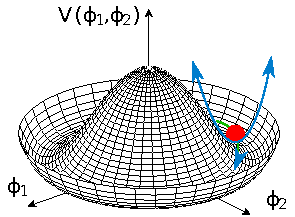
\includegraphics[scale=2]{images/higgspotential.pdf}
	\end{center}
	\caption{Potencial de Higgs: desde la perspectiva de la
        cima el potencial es sim\'etrico de rotaci\'on.
        Sin embargo, desde la perspectiva de la bola el potencial
        parece no presentar dicha simetr\'ia, esto es el ``rompimiento
        espont\'aneo de simetr\'ia''. Las fluctuaciones {\em tangenciales}
        del campo a lo largo del c\'irculo de m\'inimos se manifiestan
        como un bos\'on de Nambu-Goldstone si la simetr\'ia es global.
        Si la simetr\'ia es local, este bos\'on de Nambu-Goldstone
        est\'a ``comido'' por un campo de norma que adquiere masa. Las
        fluctuaciones {\em radiales}, perpendiculares al c\'irculo de
        m\'inimos, se manifiestan como una part\'icula masiva. Si
        tratamos con el potencial de Higgs como ocurre en el Modelo
        Est\'andar, esta part\'icula masiva es el famoso bos\'on de
        Higgs.}
\label{sombrero}        
\vspace*{-2mm}
\end{figure}

Ya hemos visto que el mecanismo tambi\'en proporciona una masa al
electr\'on, y de la misma manera aplica al mu\'on, tau\'on y a
todos los cuarks. ?`Y qu\'e pasa con el campo de Higgs?
Sabemos que 3 de sus 4 componentes ser\'ian bosones de
Nambu-Goldstone que desaparecen, pero est\'a la cuarta componente
todav\'ia, que corresponde a la fluctuaci\'on radial, es decir,
a una part\'icula masiva. Su existencia es una predicci\'on del
mecanismo de Higgs, y en este aspecto el segundo art\'iculo de Higgs
de 1964 era algo m\'as expl\'icito que los otros trabajos originales.
Esto era en el contexto de modelos juguete todav\'ia, pero una vez se
aplic\'o a un modelo fenomenol\'ogico, se concluy\'o que dicha
{\em part\'icula de Higgs} tendr\'ia que ser observable. 

La teor\'ia no predice la masa de la part\'icula de Higgs, $M_{\rm H}$
(se pueden derivar cuotas solamente que eran tema de discusi\'on durante
muchos a\~nos), por lo que la b\'usqueda experimental era dif\'icil.
Al inicio del siglo XXI, los experimentos del
Gran Colisionador de Leptones y Protones (LEP) del CERN demostraron
que tiene que tener una masa de $M_{\rm H} > 114\, {\rm GeV}$. Entonces se
sab\'ia que tiene que ser muy pesado (si existe), tal que su creaci\'on
requiere colisiones de altas energ\'ias. Esto tambi\'en implica que
su tiempo de vida es muy corto, decae en promedio en $10^{-22}$
segundos, y no puede dejar trazas en ning\'un detector.

Un experimento tiene que capturar los productos de su decaimiento
que permiten la reconstrucci\'on de la part\'icula de Higgs como
estado intermediario, o ``resonancia'' -- por muy poco tiempo --
en una colisi\'on a
altas energ\'ias. El an\'alisis de las part\'iculas que resultan al
final del proceso permiten reconstruir las propiedades de la
part\'icula de Higgs, en particular su masa de $M_{\rm H} = 125\,
{\rm GeV}$ y su esp\'in 0, que confirma que se trata de una part\'icula
escalar.

En el canal m\'as limpio que fue observado, el decaimiento del la
part\'icula de Higgs termina con dos fotones, un estado final que
no ser\'ia posible si, por ejemplo, la part\'icula original
ten\'ia esp\'in 1, como Landau hab\'ia demostrado \cite{Landau}.
Pero los experimentos ATLAS y CMS estudiaron (independientemente)
muchos m\'as decaimientos en gran detalle -- como, por ejemplo,
con un estado final de cuatro leptones -- y no dejan ninguna duda
de la existencia de la part\'icula de Higgs, y del mecanismo
correspondiente.


\begin{figure}
\centering
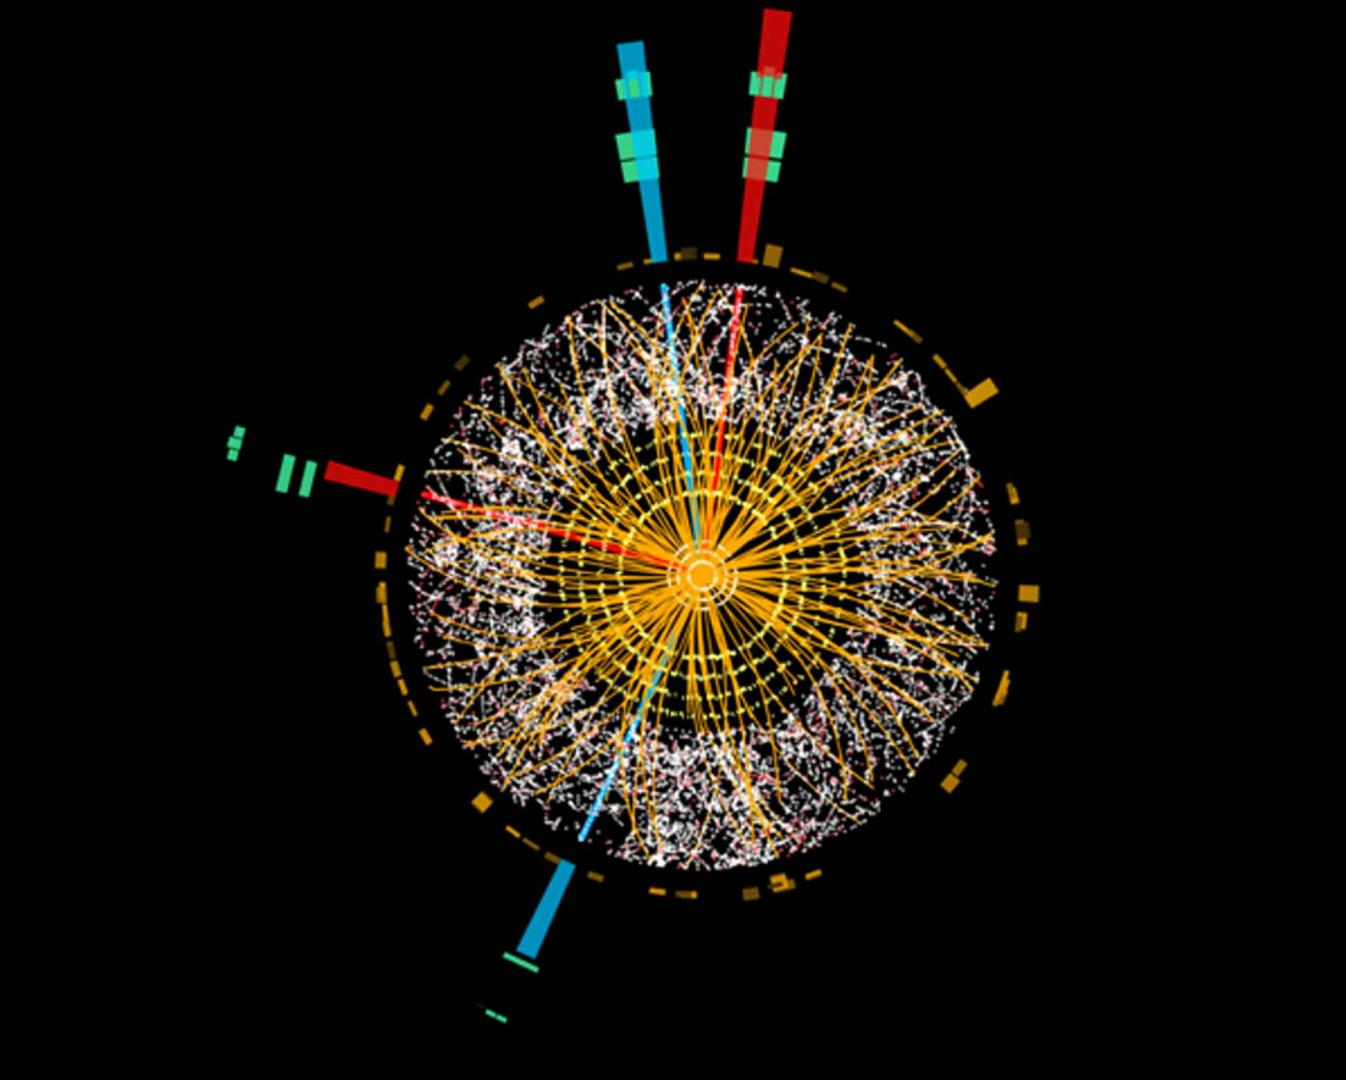
\includegraphics[scale=0.2]{images/atlas-higgs.jpg}
\caption{Canales posibles del decaimiento del bos\'on de
Higgs es cuando decae a dos bosones $Z$ que a su vez decaen cada
uno en un par lepton-antilepton. 
En la imagen observamos 4 leptones (l\'ineas rojas y azules) que
posiblemente hayan sido producidas por el decaimiento del bos\'on de Higgs.}
\end{figure}

\begin{figure}
\centering
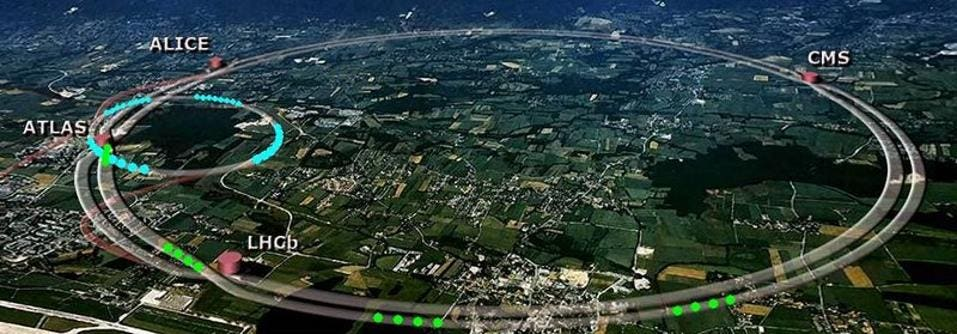
\includegraphics[scale=0.4]{images/lhc.jpg}
\caption{El Gran Colisionador de Hadrones (LHC por sus siglas en
ingl\'es) se encuentra ubicado en la regi\'on fronteriza entre
Francia y Suiza.
Sus cuatro experimentos principales se llaman ATLAS y CMS (que
de manera independiente encontraron evidencia de la existencia
del bos\'on de Higgs), ALICE (con fuerte participaci\'on mexicana)
y LHCb.}
\end{figure}

Esto representa un \'exito espectacular de la f\'isica de part\'iculas
elementales. A\'un as\'i, no todo est\'a resuelto todav\'ia. Desde la
perspectiva conceptual, se queda el {\em problema de la jerarqu\'ia}
y respecto a la fenomenolog\'ia, el mecanismo de Higgs no explica
el origen de todas las masas que obervamos. Terminamos con
comentarios breves sobre estos asuntos:

\begin{itemize}

\item {\em Problema de la jerarqu\'ia:} Si empezamos con un sistema
cl\'asico (sin efectos cu\'anticos) y suponemos una masa $m_{\rm H}^{(0)}$
en la magnitud de las masas de otras part\'iculas,
es natural que las correcciones cu\'anticas suben dicha masa
dr\'asticamente, a un valor $m_{\rm H}$ del orden de la ``escala de
Planck'' (determinada por la constante de la gravitaci\'on).
Pero esto conduce a un valor de $m_{\rm H}$ muy alto, t\'ipicamente
como $10^{17}$ veces su valor observado.

Lo que se podr\'ia hacer es suponer un valor de $m_{\rm H}^{(0)}$
extremadamente negativo, as\'i que el efecto cu\'antico
se cancela casi totalmente, y se queda un resto diminuto
de 125\,GeV. Pero esta aproximaci\'on -- con una cancelaci\'on
entre dos contribuciones tremendas que deja un resto diminuto --
no parece natural. Esto es conocido como el ``problema de la
jerarqu\'ia''. Sin embargo, no es una paradoja, se puede llegar
de manera consistente a 125\,GeV, y la pregunta de qu\'e tan
grave es este problema es un poco filos\'ofica.

\item Los {\em neutrinos} (descritos con el s\'imbolo $\nu$) tienen
un papel especial: en la forma tradicional del Modelo
Est\'andar se supuso que ten\'ian masa cero, $M_{\nu} =0$,
y que solamente exist\'ia el neutrino con quiralidad izquierda,
$\nu_L$.

Esto es consistente en teor\'ia, pero a finales del siglo XX
se observ\'o que los neutrinos s\'i tienen una peque\~na masa,
$m_{\nu}>0$ -- repetimos que Ref.\ \cite{neutrinos} presenta una
revisi\'on semi-divulgativa del tema.

De primera vista, conforme con nuestra descripci\'on anterior,
parece inevitable que exista el neutrino derecho, $\nu_R$.  
Esto permite la aplicaci\'on del mecanismo de Higgs para los
neutrinos, y adem\'as otro tipo de masa, solamente para el
$\nu_R$, conocido como ``masa de Majorana''.

Sin embargo, el $\nu_R$ no es observado, y su existencia no
es realmente inevitable: podemos construir una t\'ermino de masa
que involucra \'unicamente el campo $\nu_L$. Este t\'ermino no
es renormalizable, pero hemos mencionado en la Secci\'on 1 que ya no
se da tanta importancia a esta propiedad. Entonces este escenario
ser\'ia la alternativa, en el marco del Modelo Est\'andar interpretado
como teor\'ia efectiva que funciona en cierto rango energ\'etico.

\item Hasta este punto, el mecanismo de Higgs explica las masas
de las part\'iculas elementales (con la posible excepci\'on de
los neutrinos), y hay otras part\'iculas como el fot\'on que se
quedan sin masa. Parece una imagen completa del origen de la masa.

Sin embargo, el mundo real es diferente: en realidad, la masa de un
objeto macrosc\'opico de nuestra vida cotidiana viene solamente
por $1 \dots 2 \, \%$ del mecanismo de Higgs, que conduce a las
masas de las cuarks.

Estas masas cotidianas consisten principalmente de masas de
nucleones (protones y neutrones) que de su parte consisten
esencialmente de energ\'ia de {\em gluones} (otras part\'iculas de
norma, que transmiten la interacci\'on fuerte): tienen masa cero,
pero son confinados al interior de un nucle\'on (u otra part\'icula
compuesta por la interacci\'on fuerte). Su energ\'ia se
manifiesta como casi toda la masa del nucle\'on, mientras que
las masas da los cuarks solamente proporcionan dicha contribuci\'on
al nivel de $\sim 1 \dots 2 \, \%$.

El interior de un nucle\'on es un sistema muy, pero muy complejo,
por mucho tiempo pareci\'o imposible calcular algo conclusivo
al respecto. Sin embargo, hace un poco m\'as de una d\'ecada 
se logr\'o calcular por ejemplo la masa del nucle\'on,
$M_N \simeq 939\,{\rm MeV}$, de primeros principios, hasta una
incertidumbre del orden de 1\,\%. Este c\'alculo captura
el despelote hiper complicado de gluones (y ``cuarks de mar'',
parejas inestables de un cuark y su anti-cuark), y el
resultado es compatible con los experimentos. La pregunta de
c\'omo estos c\'alculos eran posibles ser\'ia tema para otro
art\'iculo $\dots$

\end{itemize}